\subsubsection{Crossroads}
\begin{figure}[h]
\centering
\nogloxy{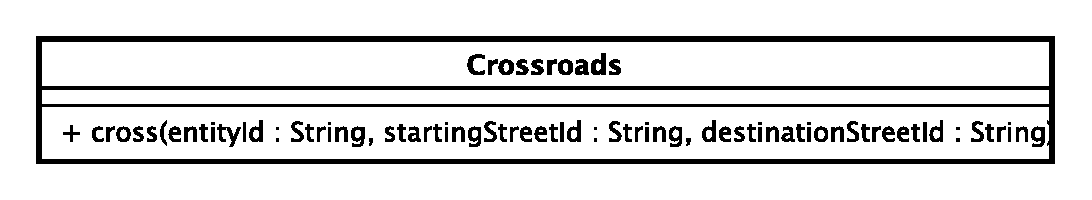
\includegraphics[scale=0.6,keepaspectratio]{diagrams/workspace/application/crossroads.eps}}
\caption{Application::Crossroads}
\end{figure}
\FloatBarrier
A crossroads is a road intersection offers the following operations:
\begin{itemize}
	\item \texttt{cross(entityId : String, startingStreetId : String, destinationStreetId : String)}
	\\Moves an entity from a street to another one
\end{itemize}
%Crossroads’ operations called by entities or roads.
\paragraph{Remarks}
\ \\A crossroads internally encapsulates the logic allows the entities to proceed neatly, i.e. way rules.